\section{Auswertung}
\label{sec:Auswertung}
\begin{figure}
  \centering
  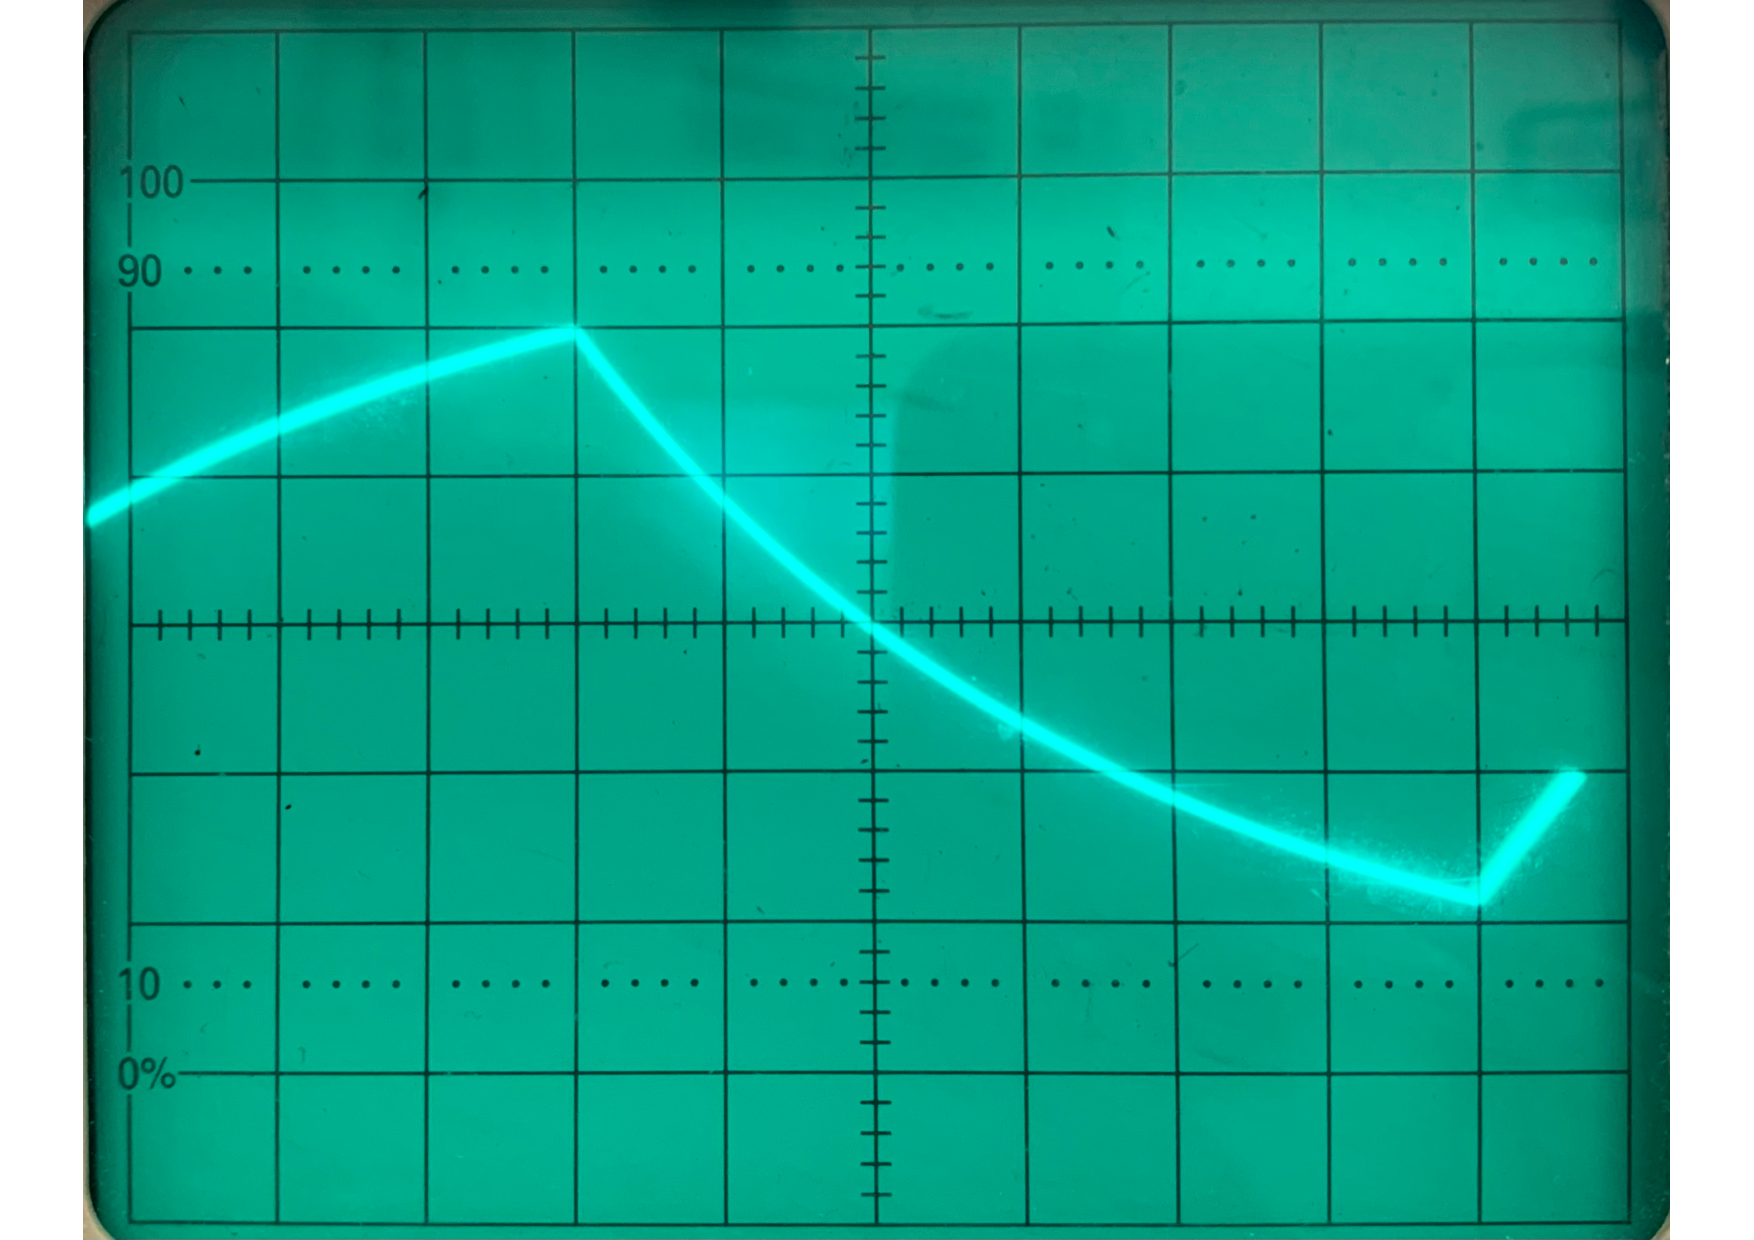
\includegraphics[height=10cm]{content/Aufgabe a - Rechteckspannung.pdf}
  \caption{Entladekurve des Kondensators mit Vorwiderstand}
  \label{fig:aufgabe a - rechteckspannung}
\end{figure}

\begin{figure}
  \begin{subfigure}{0.48\textwidth}
    \centering
    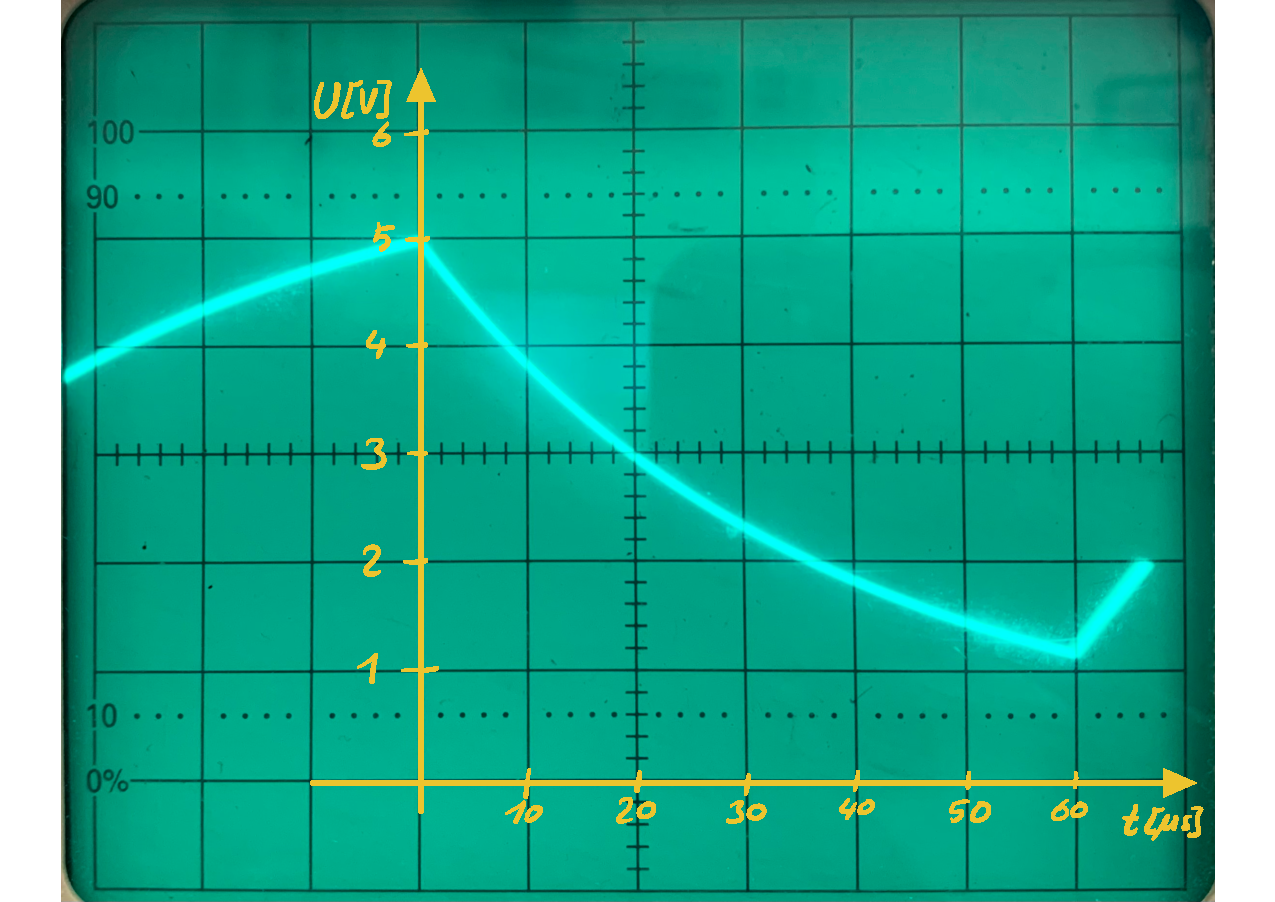
\includegraphics[height=5cm]{content/Aufgabe a - Gitter.pdf}
    \caption{Entladekurve mit Koordinatensystem}
    \label{fig:aufgabe a - gitter}
  \end{subfigure}
  \hfill
  \begin{subfigure}{0.48\textwidth}
    \centering
    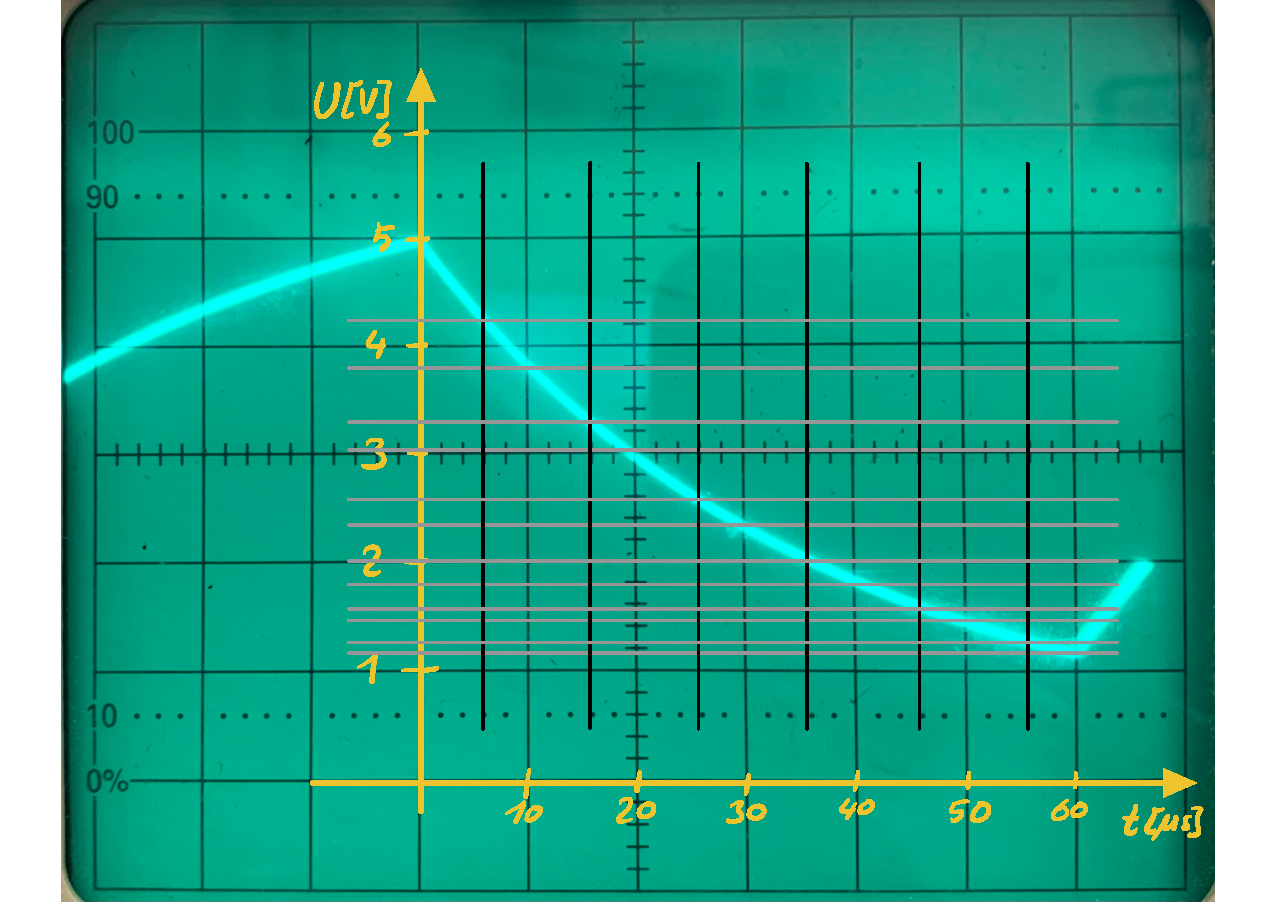
\includegraphics[height=5cm]{content/Aufgabe a - Hilfslinien.pdf}
    \caption{Entladekurve mit Hilfslinien}
    \label{fig:aufgabe a - hilfslinien}
  \end{subfigure}
  \caption{Entladekurve mit eingezeichnetem Koordinatensystem und Hilfslinien. Die %
    Skalierung wurde vorher durch Messung der Spannung der Rechteckspannung ermittelt.}
  \label{fig:aufgabe a - gitter und hilfslinien}
\end{figure}

\begin{table}
  \centering
  \caption{Darstellung der Messwertpaare, welche aus \autoref{fig:aufgabe a - gitter und hilfslinien} abgelesen wurden.}
  \label{tab:aufgabe a}
  \begin{tabular}{c c}
    \toprule
    $f$ [Hz] & $U$ [V] \\
    \midrule
    0 &  5,0 \\
    6	&  4,2 \\
    10 & 3,8 \\
    16 & 3,3 \\
    20 & 3,0 \\
    26 & 2,6 \\
    30 & 2,3 \\
    36 & 2,0 \\
    40 & 1,8 \\
    46 & 1,6 \\
    50 & 1,4 \\
    56 & 1,2 \\
    60 & 1,1 \\
    \bottomrule
  \end{tabular}
\end{table}

\begin{table}
  \centering
  \caption{Darstellung der Messwerte zu den Aufgabenteilen b) und c)}
  \label{tab:aufgaben cd}
  \begin{tabular}{c c c c}
    \toprule
    $f$ [Hz] & $A$ [V] & $a$ [$\symup{\mu}$s] & $b$ [$\symup{\mu}$s] \\
    \midrule
    50  &	2,8	& 0	& 20000 \\
    100 &	2,65 & 100 & 10000 \\
    150 &	2,6 &	100 & 6500 \\
    200 & 2,6 &	100 & 5000 \\ 
    500 &	2,6 &	100	& 2000 \\
    1000 & 2,5 &	100 & 1000 \\
    1500 & 2,3 & 55 & 630 \\
    2000 & 2,05 &	50 & 500 \\
    3000 & 1,8 & 44 & 330 \\
    4000 & 1,5 & 40 & 250 \\
    5000 & 1,1 & 36 & 200 \\
    10000 &	0,68 & 22 & 100 \\
    20000 &	0,3 & 12 & 52 \\
    30000 &	0,22 & 8 & 34 \\
    50000 &	0,14 & 4,9 & 20 \\
    100000 & 0,07 &	2,5 & 10 \\
    \bottomrule
  \end{tabular}
\end{table}

\begin{figure}
  \centering
  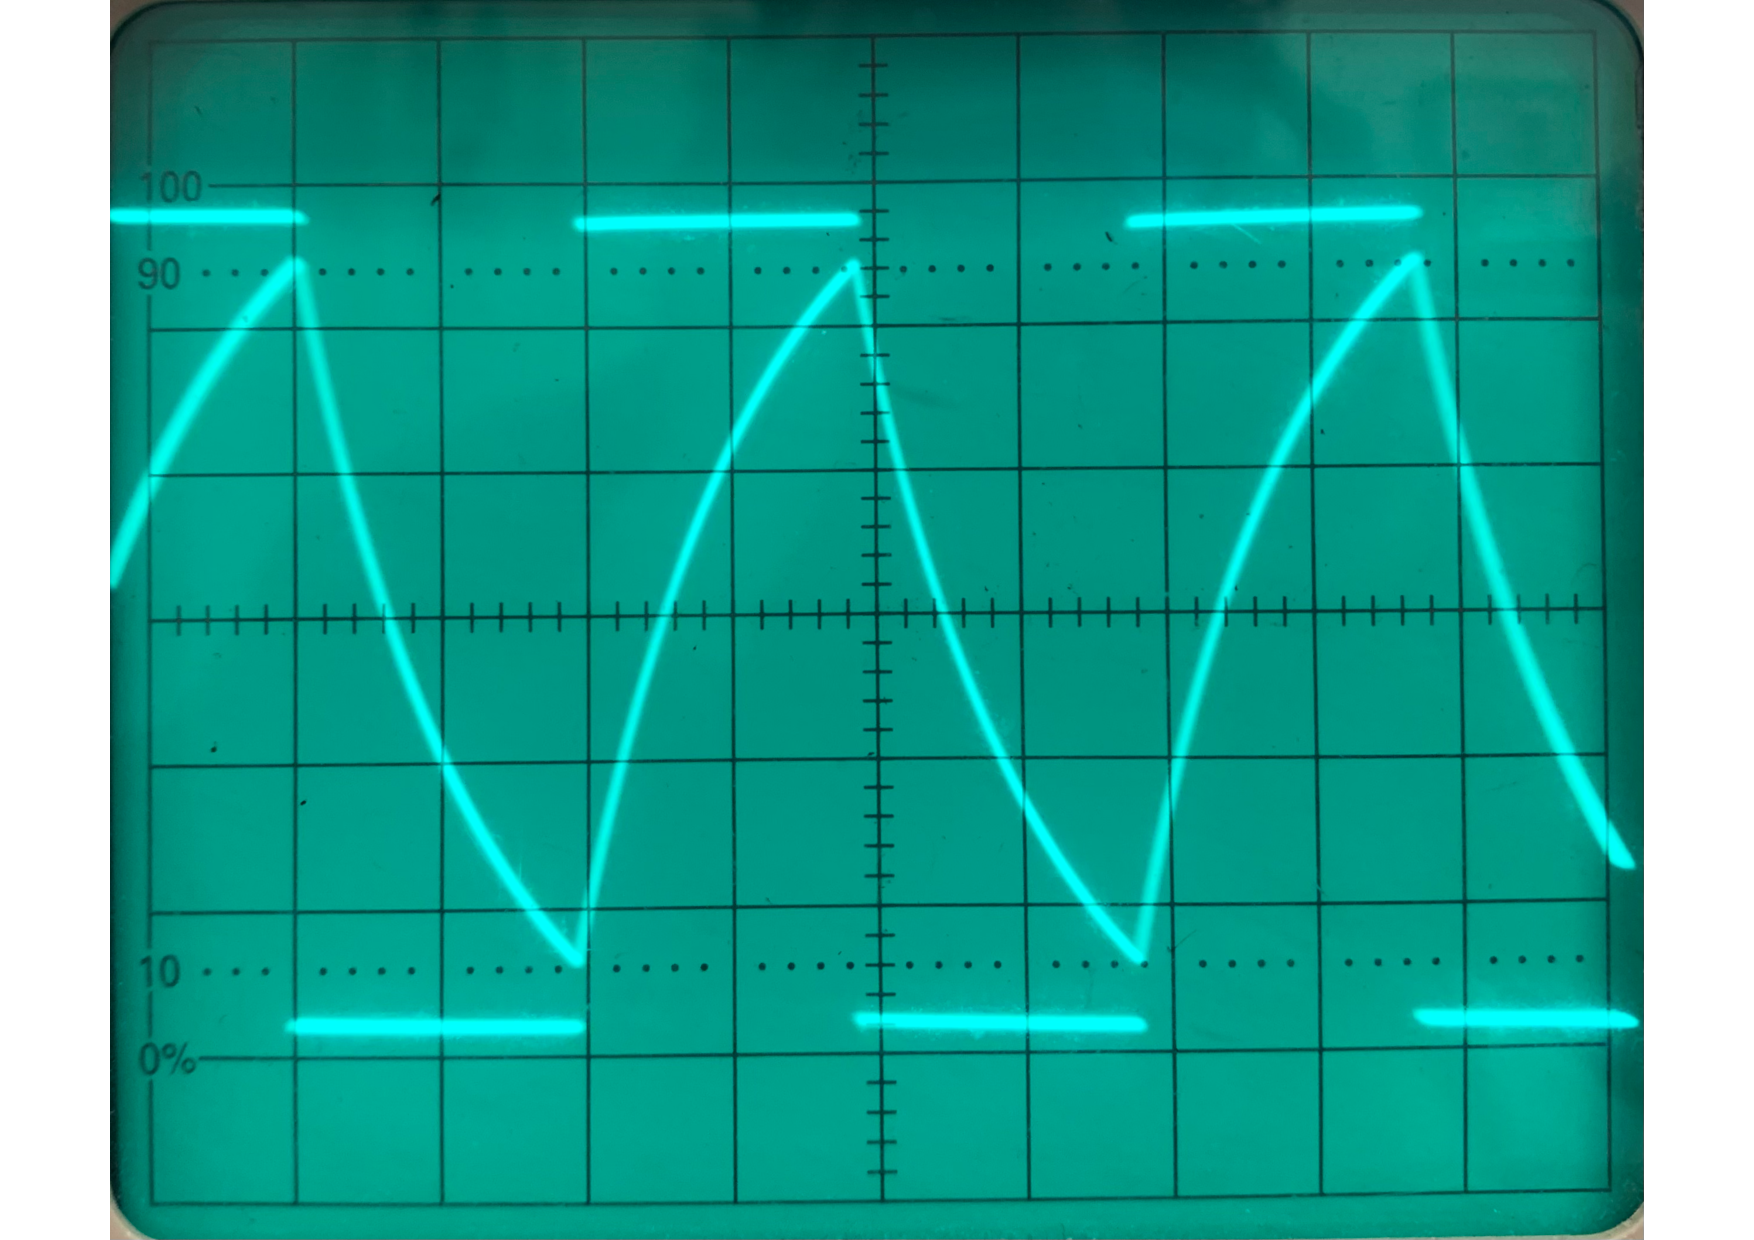
\includegraphics[height=10cm]{content/Aufgabe d - Rechteckspannung.pdf}
  \caption{Rechteckspannung $U_{0}$ und Kondensatorspannung mit $f=5$kHz}
  \label{fig:aufgabe d - rechteckspannung}
\end{figure}

\begin{figure}
  \centering
  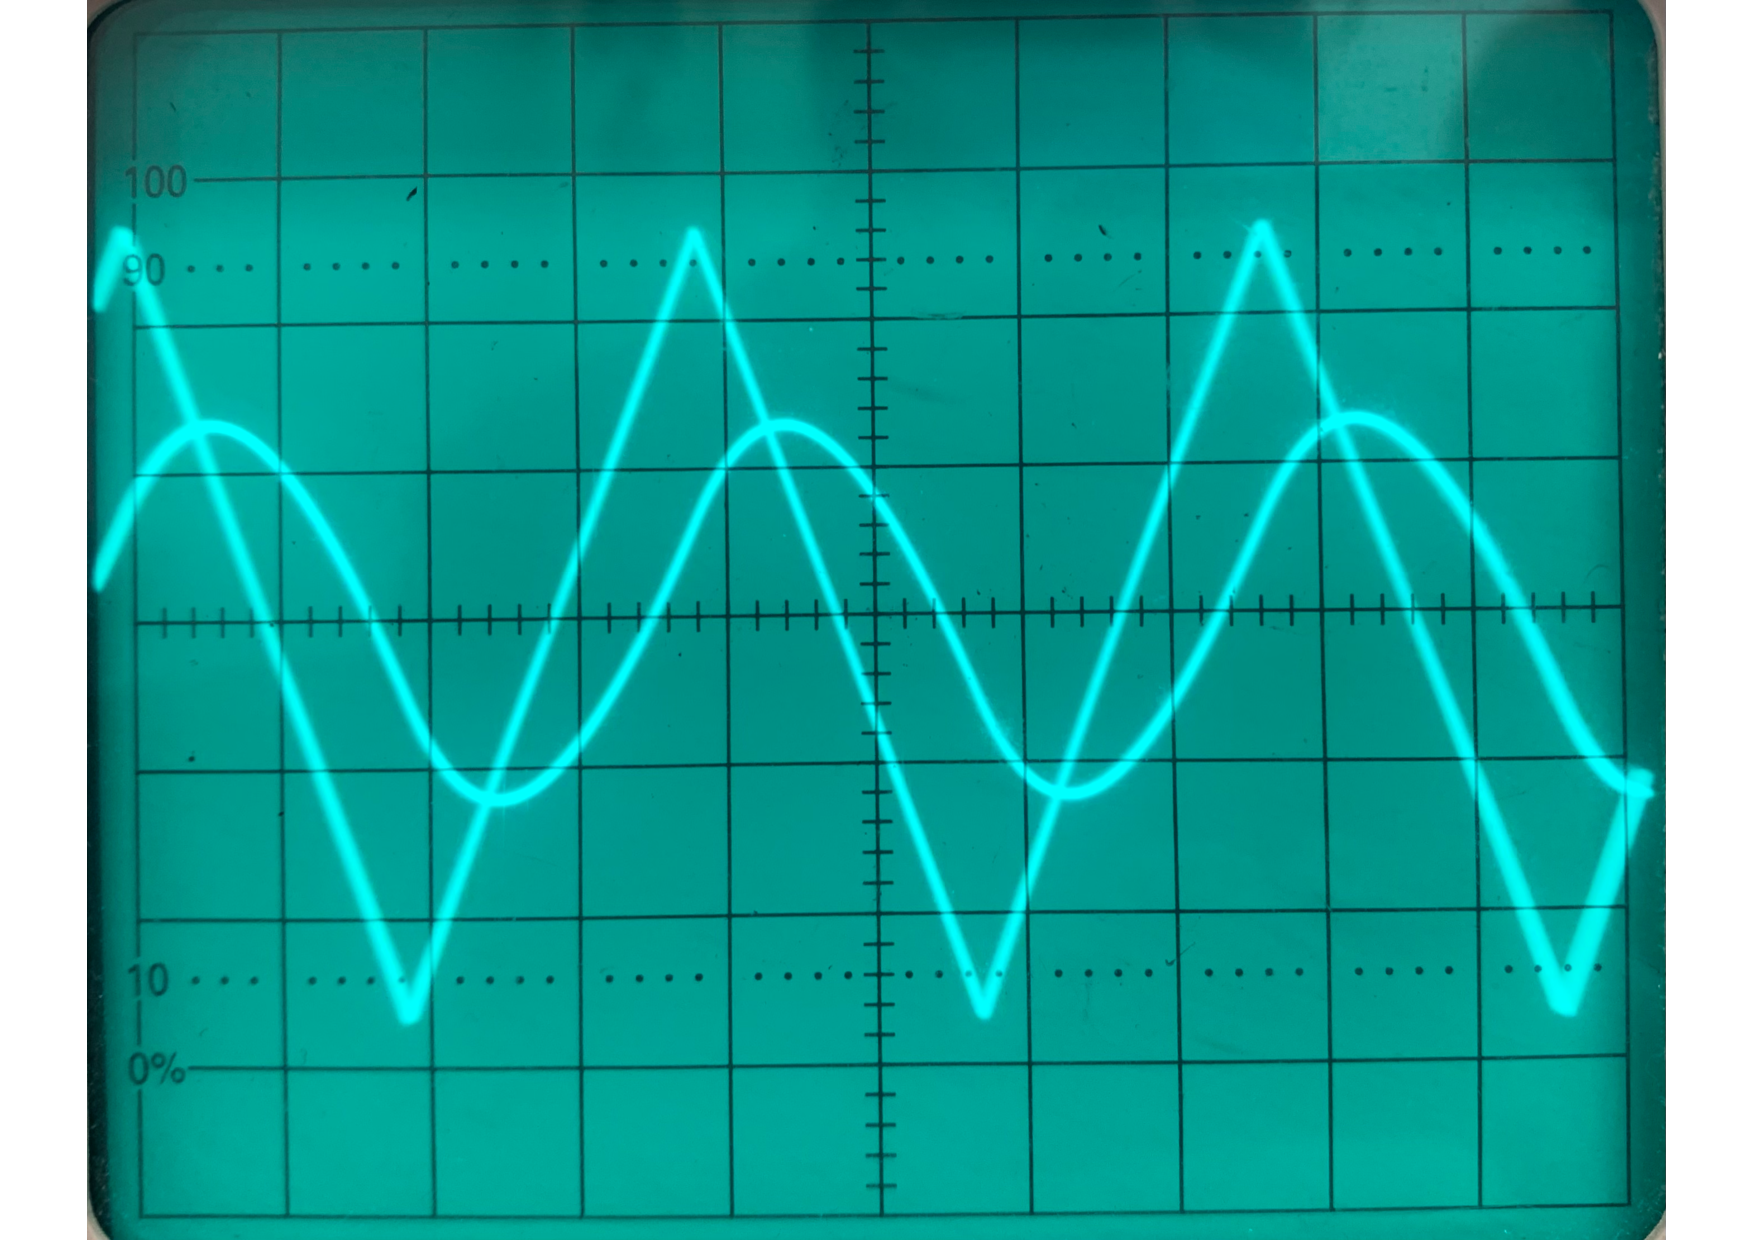
\includegraphics[height=10cm]{content/Aufgabe d - Dreieckspannung.pdf}
  \caption{Dreieckspannung $U_{0}$ und Kondensatorspannung mit $f=5$kHz}
  \label{fig:aufgabe d - dreieckspannung}
\end{figure}

\begin{figure}
  \centering
  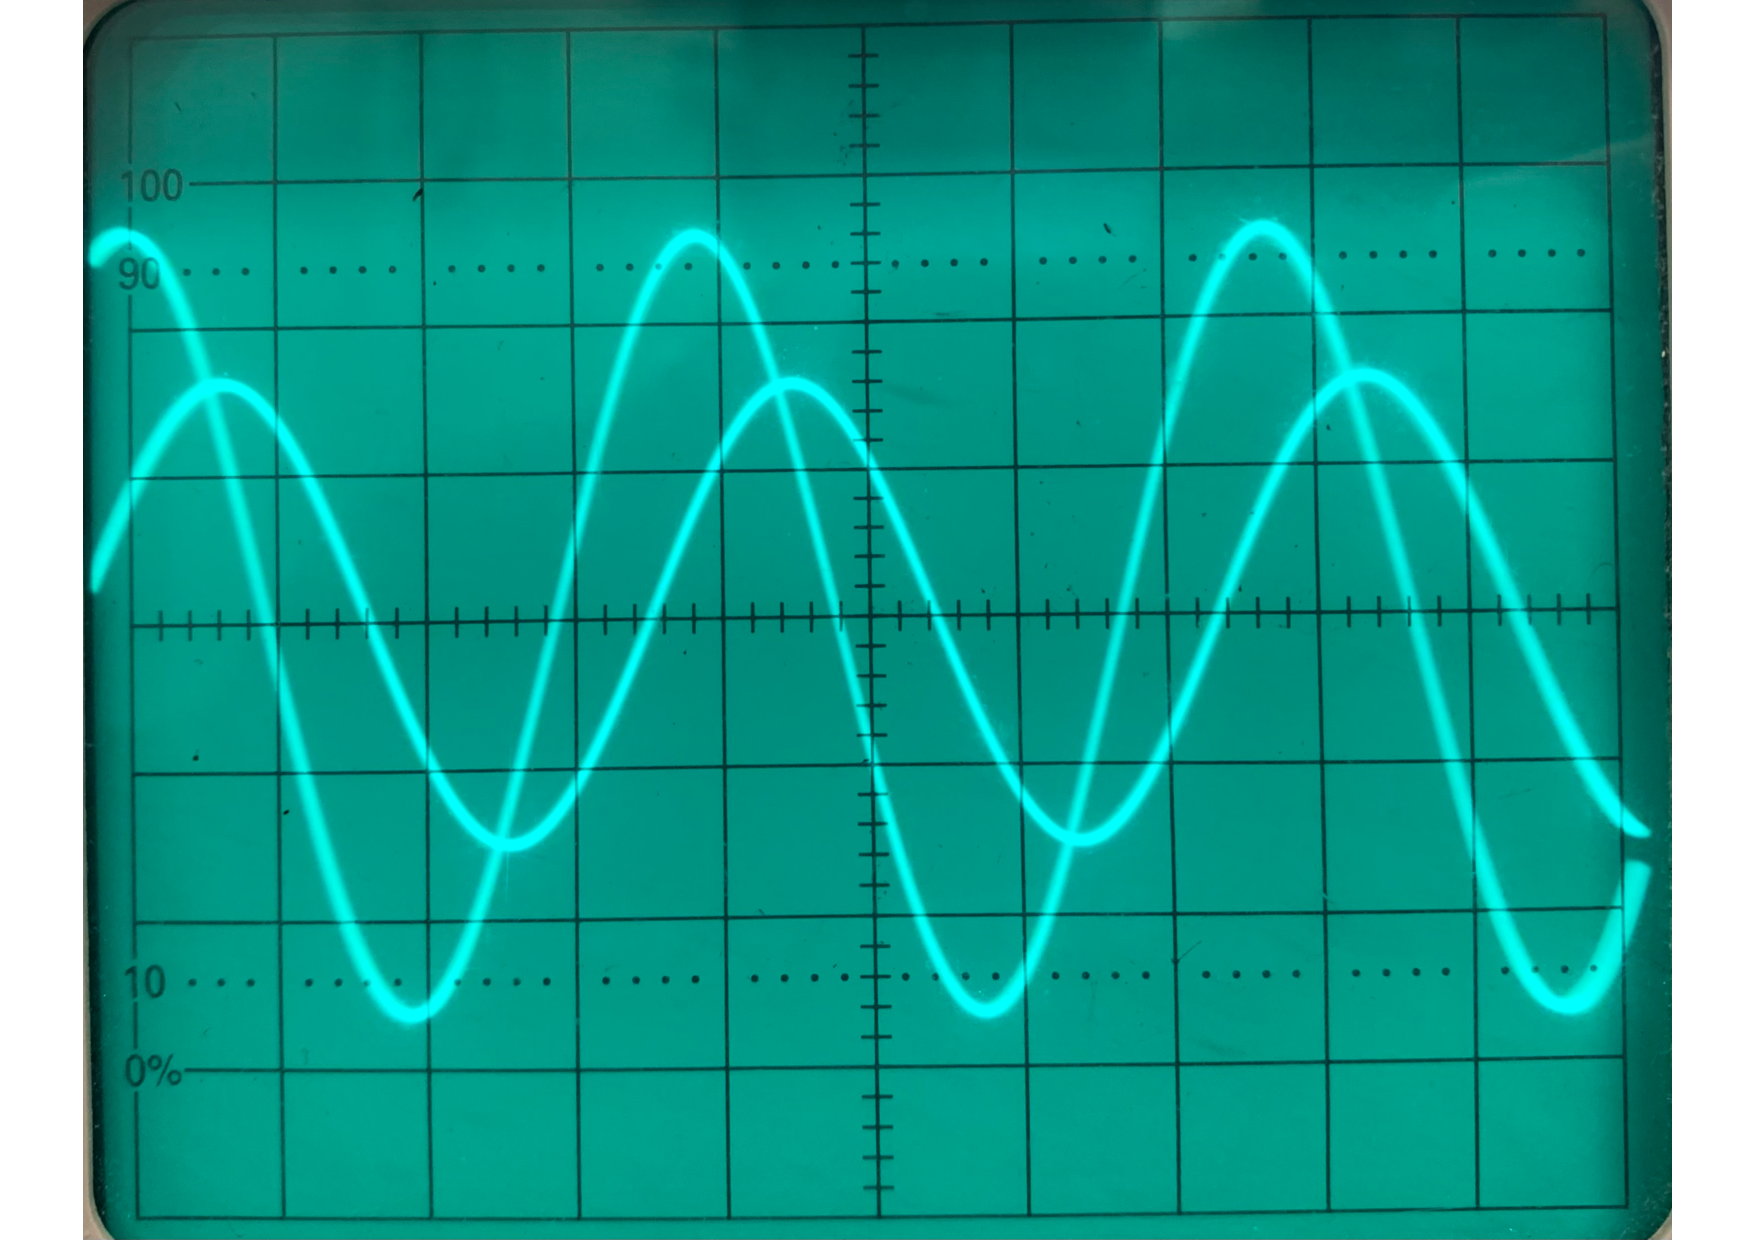
\includegraphics[height=10cm]{content/Aufgabe d - Sinusspannung.pdf}
  \caption{Sinusspannung $U_{0}$ und Kondensatorspannung mit $f=5$kHz}
  \label{fig:aufgabe d - sinusspannung}
\end{figure}
